% \section{Análisis de Soluciones Similares}

Antes de proceder con la planificación del proyecto, es un buen ejercicio analizar las alternativas similares que actualmente existen en el mercado. Como se menciona en la sección de \nameref{ch:contexto}, la mayoría de otras webs ofrecen estadísticas muy básicas, como visualizar los \textit{top géneros}, \textit{artistas} y \textit{álbumes} del usuario, además de su \textit{historial de reproducción} más reciente. Cada una de estas funcionalidades corresponde a llamadas directas a la \textit{Web API} de \textit{Spotify}, siendo estadísticas triviales de implementar, con una mínima necesidad de procesamiento de datos.

\vspace{0.5cm}

\begin{table}[htbp]
    \centering
    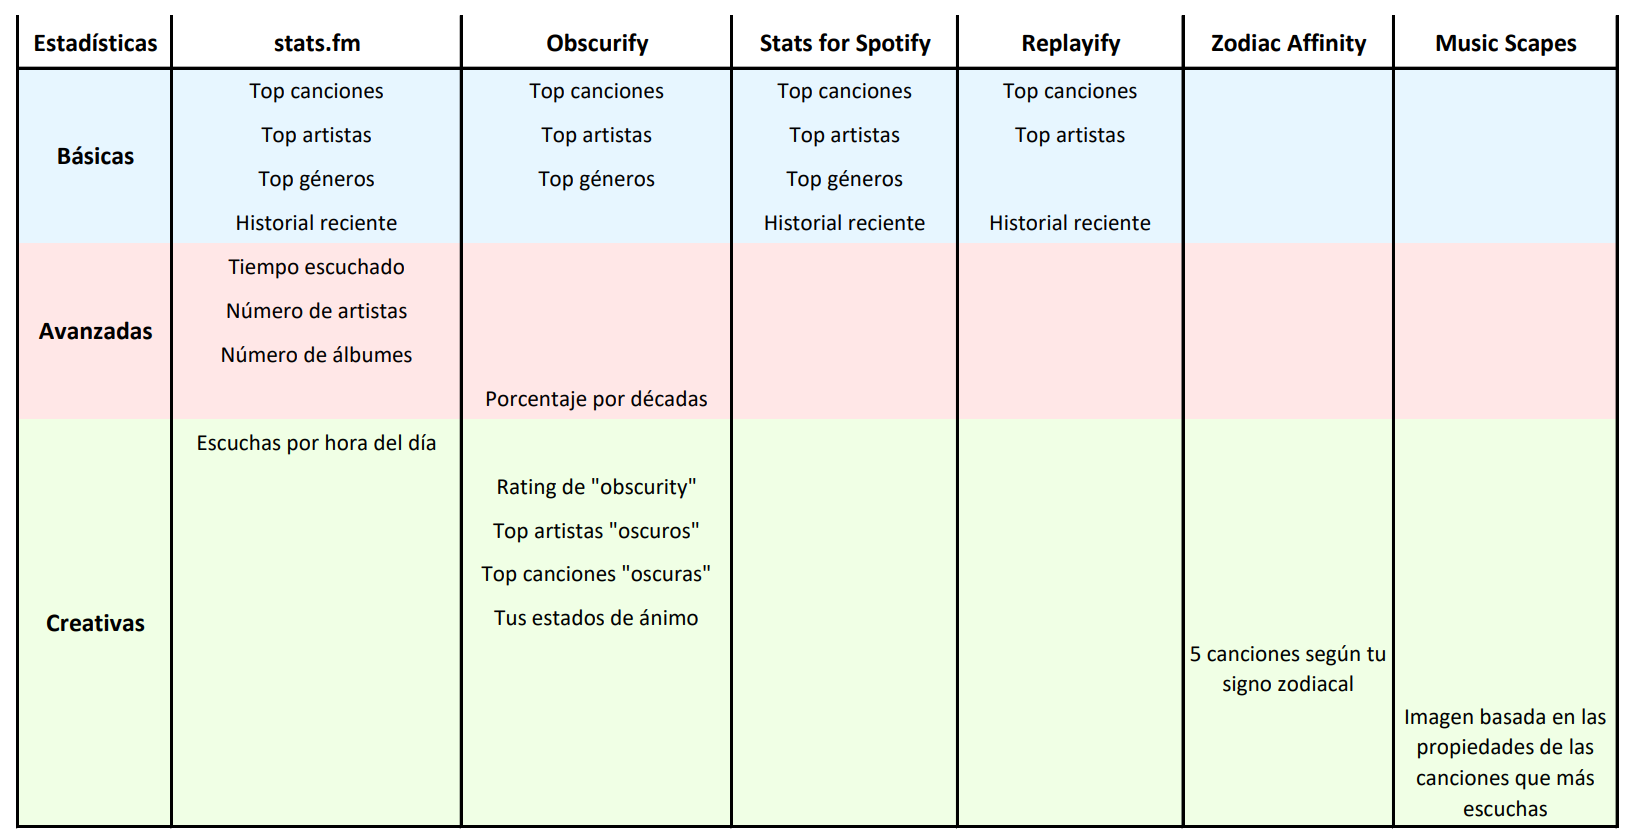
\includegraphics[width=\textwidth]{figures/tabla_comparativa.png}
    \caption{Comparativa de funcionalidades ofrecidas por otros servicios afines.}
    \label{tab:comparativa}
\end{table}

\vspace{0.5cm}

Una de las opciones más populares es la aplicación web \textit{stats.fm}\footnote{stats.fm: \url{https://spotistats.app/}}. Esta ofrece las funcionalidades básicas mencionadas a todos los usuarios, pero, mediante un plan de pago, se habilitan gráficas más avanzadas. Estas gráficas no se obtienen directamente de la API, sino que requieren que el usuario descargue manualmente los datos históricos guardados por \textit{Spotify} y los suba a la página web como un archivo comprimido. De esta manera, se generan estadísticas relativamente más complejas, pero que aún carecen de ``creatividad'' en su presentación.

% \begin{figure}[htbp]
%     \centering
%     
\includegraphics[width=0.33\textwidth]{figures/stats.fm_logo.png}
%     \caption{Logo de stats.fm.}
%     \label{fig:stats.fm_logo}
% \end{figure}

Otro servicio notable es \textit{Obscurify}\footnote{Obscurify: \url{https://www.obscurifymusic.com/}}, que se centra en la ``oscuridad'' o ``rareza'' de la música que el usuario escucha. El concepto principal de \textit{Obscurify} es identificar las canciones y artistas que son menos populares entre otros usuarios de \textit{Spotify}, clasificándolos como más ``oscuros''. Esta funcionalidad permite que el usuario se sienta especial al escuchar música que no es común. Sin embargo, su enfoque está limitado en su mayoría a este concepto, lo que deja fuera otras formas de visualización o análisis más amplios y variados.

% \begin{figure}[htbp]
%     \centering
%     
\includegraphics[width=0.33\textwidth]{figures/obscurify_logo.png}
%     \caption{Logo de Obscurify.}
%     \label{fig:obscurify_logo}
% \end{figure}

\begin{figure}[htbp]
    \centering
    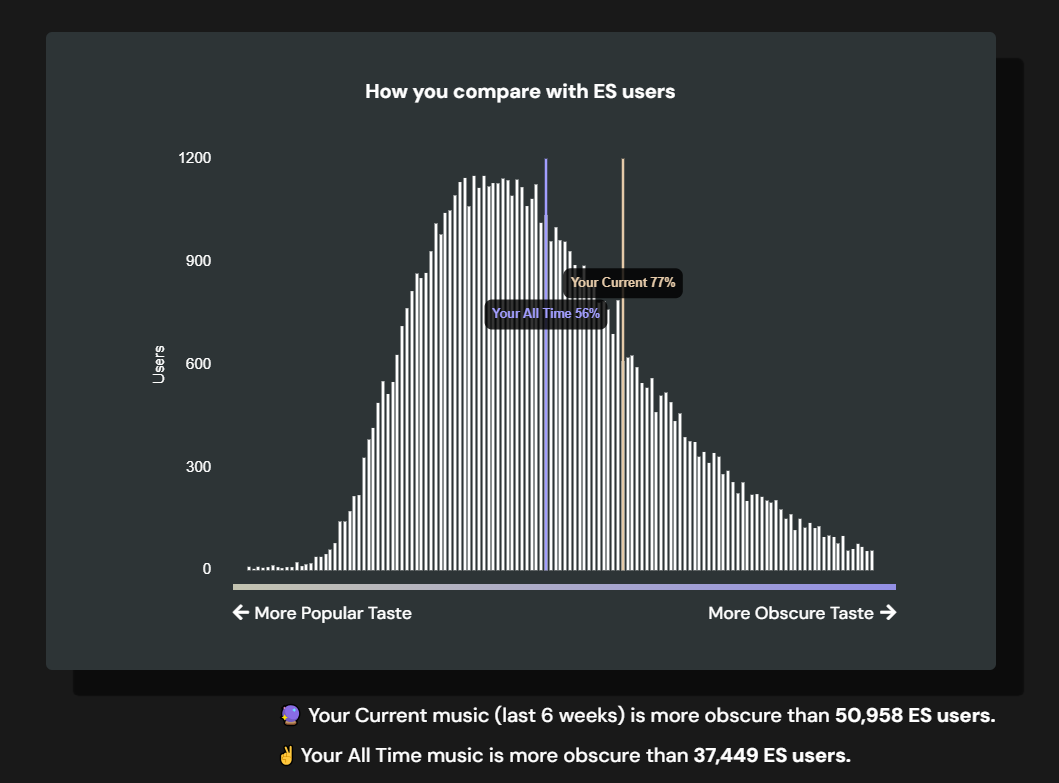
\includegraphics[width=0.67\textwidth]{figures/obscuify_stat.png}
    \caption{Estadística de ``oscuridad'' de \textit{Obscurify}.}
    \label{fig:obscurify_stat}
\end{figure}

Además de estas páginas principales, existen otras que se enfocan toda su funcionalidad en una única característica original, sin ofrecer mucho más. Dos ejemplos destacados son \textit{Zodiac Affinity}\footnote{Zodiac Affinity: \url{https://zodiacaffinity.eu/}} y \textit{MusicScapes}\footnote{MusicScapes: \url{https://musicscapes.herokuapp.com/}}. La primera genera una recomendación de cinco canciones en base a los hábitos de escucha del usuario y su signo zodiacal, mientras que la segunda crea de manera procedural una imagen basada en diferentes propiedades de las canciones que el usuario ha escuchado recientemente. Estas páginas no ofrecen ninguna funcionalidad adicional, limitándose a esa única característica. Aunque hay otros servicios similares, he elegido estos dos ejemplos por su aspecto más ``acabado'', ya que muchas otras alternativas se presentan más como una prueba de concepto o una demo, en lugar de páginas completamente desarrolladas.

\begin{figure}[htbp]
    \centering
    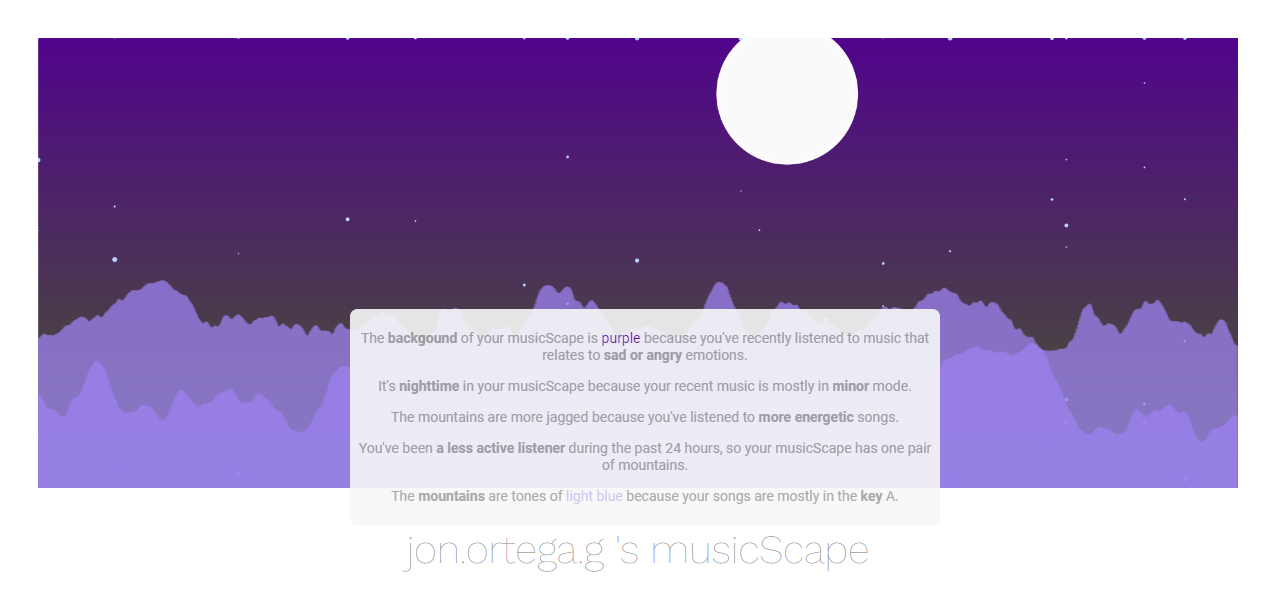
\includegraphics[width=\textwidth]{figures/music_scapes_ejemplo.png}
    \caption{Imagen generada por MusicScapes.}
    \label{fig:musicscapes_ejemplo}
\end{figure}
